% !TEX root = Theo_III.tex


\chapter{Elektrische Felder in Materie}

In diesem Kapitel werden die makroskopischen Gleichungen der Elektrostatik in Materie beschrieben und erläutert.



\section{Mikroskopische Gleichungen der Elektrostatik und Mittelung\label{sec:mikroskopische_gleichungen_der_elektrostatik}}

Bis jetzt haben wir nur freie Ladungen betrachtet. Die Ladungsdichte $\rho \left(\vec {r}\right)$ erzeugt ein elektrisches Feld $\vec {E}(\vec r)$. In Materie sind zusätzlich auch gebundene Ladungen vorhanden, die mit dem Feld wechselwirken. Das können (nach außen hin elektrisch neutrale) Atome, geladenen Ionen, permanente Dipole (oder Multipole) sein (z.B. $\mathrm{H}_{2}\mathrm{O}$), sowie Dipole sein, die durch ein äußeres elektrisches Feld induziert werden.

Um diese Wechselwirkung zu beschreiben, wird eine Mittelung der mikroskopischen Gleichungen
\begin{equation*}
	\divg \vec {e}=\frac{1}{\varepsilon _{0}}\rho \left(\vec {r}\right),\quad \rot \vec {e}=0
\end{equation*}
durchgeführt. Wir haben bisher einzelne Ladungen durch $\delta $-Funktionen in der Ladungsdichte beschrieben. Dadurch kommt es zu starken räumlichen Ladungsschwankungen. Für eine makroskopische Betrachtung in Größenordnungen von Nanometern wenden wir eine räumliche Mittelung bzw. Glättungsfunktion auf die Ladungsdichteverteilung an.




\subsection{Glättungsfunktion}

Um eine stark variierende Funktion $F\left(\vec {r},t\right)$ zu mitteln, wird sie mit einer sogenannten Glättungsfunktion $f$ gefaltet. Dabei kann es sich z.B. um eine Gauß-Funktion handeln:
\begin{equation*}
	F\left(\vec {r},t\right) \xrightarrow{\text{Mittelung}} \left\langle F\left(\vec {r},t\right)\right\rangle =\int f\left(\left| \vec {r}-\vec {r}'\right| \right)F\left(\vec {r}',t\right)\diffa[3]{\vec{r}'}
\end{equation*}
Für eine Punktladung $F\left(\vec {r}\right)=F_{0}\delta \left(\vec {r}-\vec {r}_{0}\right)$ ist dann zum Beispiel $\left\langle F\right\rangle =F_{0}f\left(\vec {r}-\vec {r}_{0}\right)$.

Für die Mittelung gelten die folgenden Eigenschaften:\begin{enumerate}
	\item Die Mittelung der konstanten Funktion $F=1$ ist genau dann konstant $1$, wenn die Glättungsfunktion über den gesamten Raum auf $1$ normiert ist,
	      \begin{equation*}
		      \left\langle 1\right\rangle =1\equivalence \int \diffa[3]{\vec{r}}f=1.
	      \end{equation*}
	\item $\partial _{i}\left\langle F\right\rangle =\left\langle \partial _{i}F\right\rangle $.
\end{enumerate}



\section{Makroskopische Gleichungen der Elektrostatik\label{sec:Makroskopische_Gleichungen_der_Elektrostatik}}

Mithilfe der Glättung kann man das makroskopische $\vec {E}$-Feld als
\begin{equation*}
	\vec {E}\left(\vec {r},t\right)=\left\langle \vec {e}\left(\vec {r},t\right)\right\rangle
\end{equation*}
schreiben. Für die Ladungsdichte erhält man
\begin{equation*}
	\left\langle \rho \left(\vec {r}\right)\right\rangle =\left\langle \rho _{f}\left(\vec {r}\right)+\rho _{b}\left(\vec {r}\right)\right\rangle =\left\langle \rho _{f}\left(\vec {r}\right)\right\rangle +\left\langle \rho _{b}\left(\vec {r}\right)\right\rangle \equiv \rho _{F}+\rho _{B}.
\end{equation*}
Die gebundenen Ladungen werden als Summe der Ladungsdichten einzelner Moleküle geschrieben:
\begin{equation*}
	\rho _{b}\left(\vec {r}\right)=\sum _{n}\rho _{n}\left(\vec {r}\right), \rho _{n}\left(\vec {r}\right)=\sum _{i}q_{i}\delta \left(\vec {r}-\vec {r}_{i}\right)=\sum _{i}q_{i}\delta \left(\vec {r}-\left(\vec {r}_{n}+\vec {r}_{ni}\right)\right)
\end{equation*}
mit neuen Bezugspunkten $\vec {r}_{n}$ für die einzelnen Moleküle. Für die Mittelung wird dann eine Taylor-Entwicklung um diese neuen Bezugspunkte $\vec {r}_{n}$ durchgeführt:
\begin{align*}
	\left\langle \rho _{n}\left(\vec {r}\right)\right\rangle & =\sum _{i}q_{i}f\left(\vec {r}-\left(\vec {r}_{n}+\vec {r}_{ni}\right)\right) \\&=\sum _{i}q_{i}\left[f\left(\vec {r}-\vec {r}_{n}\right)-\vec {r}_{ni}\cdot \nabla f\left(\vec {r}-\vec {r}_{n}\right)+\frac{1}{2}\left(\vec {r}_{ni}\right)_{k}\left(\vec {r}_{ni}\right)_{l}\nabla _{k}\nabla _{l}f\left(\vec {r}-\vec {r}_{n}\right)+\ldots \right]
\end{align*}
Daraus können die molekularen Dipolmomente bestimmt werden:
\begin{align*}
	q_{n}                            & =\sum _{i}q_{i}                                                              & \text{(Molekulare Ladung)}           \\
	\vec {p}_{n}                     & =\sum _{i}q_{i}\vec {r}_{ni}                                                 & \text{(Molekulares Dipolmoment)}     \\
	\left(\mathrm{Q}_{n}\right)_{kl} & =3\sum _{i}q_{i}\left(\vec {r}_{ni}\right)_{k}\left(\vec {r}_{ni}\right)_{l} & \text{(Molekulares Quadrupolmoment)}
\end{align*}
(vgl. Multipolmomente einer kontinuierlichen Ladungsverteilung, aber hier jetzt diskret). Insgesamt ergibt sich eine Verschmierung punktförmiger molekularer Multipole:
\begin{align*}
	\left\langle \rho _{n}\left(\vec {r}\right)\right\rangle & =q_{n}f\left(\vec {r}-\vec {r}_{n}\right)-\vec {p}_{n}\cdot \nabla f\left(\vec {r}-\vec {r}_{n}\right)+\frac{1}{6}\left(\mathrm{Q}_{n}\right)_{kl}\nabla _{k}\nabla _{l}f\left(\vec {r}-\vec {r}_{n}\right) \\&=\left\langle q_{n}\delta \left(\vec {r}-\vec {r}_{n}\right)\right\rangle -\nabla \cdot \left\langle p_{n}\delta \left(\vec {r}-\vec {r}_{n}\right)\right\rangle +\frac{1}{6}\nabla _{k}\nabla _{l}\left\langle \left(\mathrm{Q}_{n}\right)_{kl}\delta \left(\vec {r}-\vec {r}_{n}\right)\right\rangle
\end{align*}
und für die gemittelte gebundene Ladungsdichte:
\begin{equation*}
	\left\langle \rho _{b}\left(\vec {r}\right)\right\rangle =\rho _{\mathrm{m}}\left(\vec {r}\right)-\nabla \cdot \vec {P}\left(\vec {r}\right)+\nabla _{k}\nabla _{l}{Q}_{\mathrm{kl}}+\ldots
\end{equation*}
mit der makroskopischen Ladungsdichte (Monopoldichte)
\begin{equation*}
	\rho _{\mathrm{m}}\left(\vec {r}\right)=\left\langle \sum _{n}q_{n}\delta \left(\vec {r}-\vec {r}_{n}\right)\right\rangle ,
\end{equation*}
der Polarisation (Dipolmomentdichte)
\begin{equation*}
	\vec {P}\left(\vec {r}\right)=\left\langle \sum _{n}\vec {p}_{n}\delta \left(\vec {r}-\vec {r}_{n}\right)\right\rangle
\end{equation*}
und so weiter.


Damit ergibt sich jetzt insgesamt die gemittelte mikroskopische Ladungsdichte
\begin{equation*}
	\left\langle \rho \left(\vec {r}\right)\right\rangle =\left\langle \rho _{f}\left(\vec {r}\right)\right\rangle +\left\langle \rho _{b}\left(\vec {r}\right)\right\rangle =\underset{\rho _{\mathrm{Ma}}\left(\vec {r}\right)}{\underbrace{\rho _{F}\left(\vec {r}\right)+\rho _{m}\left(\vec {r}\right)}}\underset{\rho _{\mathrm{Mi}}\left(\vec {r}\right)}{\underbrace{-\nabla \cdot \vec {P}\left(\vec {r}\right)+\nabla _{k}\nabla _{l}Q_{kl}\left(\vec {r}\right)}}
\end{equation*}
und es folgt für die makroskopischen Feldgleichungen
\begin{align*}
	\left\langle \divg \vec {e}\right\rangle & =\frac{1}{\varepsilon _{0}}\left\langle \rho \left(\vec {r}\right)\right\rangle ,\quad \left\langle \rot \vec {e}\right\rangle =\vec {0}                                                                                                                                                               \\
	\divg \vec {E}                           & =\frac{1}{\varepsilon _{0}}\left(\rho _{\mathrm{Ma}}\left(\vec {r}\right)+\rho _{\mathrm{Mi}}\left(\vec {r}\right)\right)=\frac{1}{\varepsilon _{0}}\left(\rho _{\mathrm{Ma}}\left(\vec {r}\right)-\nabla \cdot \vec {P}\left(\vec {r}\right)+\nabla _{k}\nabla _{l}Q_{kl}\left(\vec {r}\right)\right)
\end{align*}
und
\begin{equation*}
	\rot \vec {E}=\vec {0}.
\end{equation*}
An dieser Stelle führen wir jetzt das sogenannte dielektrische Verschiebungsfeld $\vec {D}$ ein:
\begin{equation*}
	\vec {D}\left(\vec {r}\right)=\varepsilon _{0}\vec {E}\left(\vec {r}\right)+\vec {P}\left(\vec {r}\right)-\nabla Q\left(\vec {r}\right)
\end{equation*}
Dabei ist die Idee, dass höhere Multipole der Ladungen jetzt in dem Hilfsfeld $\vec {D}$ stecken. In der Regel wird übrigens bereits das Quadrupolmoment vernachlässigt.

Damit können die makroskopischen Feldgleichungen jetzt geschrieben werden als
\begin{equation*}
	\boxed{\divg \vec {D}=\rho _{\mathrm{Ma}}\left(\vec {r}\right), \quad\rot \vec {E}=0.}
\end{equation*}
Die Quellen des dielektrischen Verschiebungsfeldes sind also die makroskopischen Ladungsdichten und nicht die höheren Multipolmomente. Außerdem ist $\vec {D}$ nur ein Hilfsfeld, das fundamentale Feld ist das elektrische Feld $\vec {E}$.

Die Polarisation $\vec {P}$ wird zur Darstellung in der Regel nach $\vec {E}$ entwickelt,
\begin{equation*}
	P_{i}\left(\vec {E}\right)=\varepsilon _{0}\chi _{ij}^{\left(1\right)}E_{j}+\varepsilon _{0}\chi _{ijk}^{\left(2\right)}E_{j}E_{k}+\ldots ,
\end{equation*}
wobei $\chi _{ij}^{\left(1\right)}, \chi _{ijk}^{\left(2\right)},\ldots $ die hier neu eingeführten elektrischen Suszeptibilitätstensoren sind. Im linearen, isotropen Medium gilt
\begin{equation*}
	\vec {P}\left(\vec {E}\right)=\varepsilon _{0}\chi \vec {E},
\end{equation*}
wobei $\chi $ ein Skalar ist. Das trifft hauptsächlich auf Gase, Flüssigkeiten und kubischen Kristalle zu. In anisotropen Medien ist $\chi ^{\left(1\right)}$ ein Tensor zweiter Stufe und für nicht-lineare Medien werden noch höhere Suszeptibilitäten $\chi ^{\left(n\right)}$ relevant, die Tensoren der Stufe $\left(n+1\right)$ sind. Diese sind besonders wichtig in der nicht-linearen Optik. Im Allgemeinen ist die Polarisation nicht parallel zum elektrischen Feld und nur im linearen und isotropen Fall ist $\vec {P}\parallel \vec {E}$.

Häufig wird auch der dielektrische Tensor $\varepsilon $ eingeführt:
\begin{equation*}
	\vec {D}\left(\vec {r}\right)=\varepsilon _{0}\vec {E}\left(\vec {r}\right)+\vec {P}\left(\vec {r}\right)\equiv \varepsilon \vec {E}\left(\vec {r}\right), \quad\varepsilon \equiv \varepsilon _{0}\left(1+\chi ^{\left(1\right)}\right)
\end{equation*}
Dieser ist uns für den linearen, isotropen Fall wiederum schon bekannt als Dielektrizitätskonstante oder Permittivität $\varepsilon _{r}=\chi +1$.

Eine andere Beschreibung erfolgt mithilfe der atomaren Polarisierbarkeit $\alpha $ (im Allgemeinen ebenfalls ein Tensor zweiter Stufe), die das molekulare Dipolmoment mit dem elektrischen Feld verbindet,
\begin{equation*}
	\vec {p}=\varepsilon _{0}\alpha \vec {E}.
\end{equation*}
Mit der Dipoldichte $n=N/V$ lässt sich die Polarisation schreiben als
\begin{equation*}
	\vec {P}=\varepsilon _{0}n\alpha \vec {E}, \quad\chi ^{\left(1\right)}=n\alpha .
\end{equation*}
Polarisation kann in einem Medium auftreten als permanente, ausgerichtete Dipole (in ferroelektrischen Materialien), die durch die Kristallstruktur bedingt sind, als induzierte Polarisation durch Ausrichtung von ungeordneten permanenten Dipolen gegen die thermische Bewegung oder durch Verschiebung von Ladungen innerhalb des Mediums (typisch für Dielektrika).



\section{Randbedingungen von Dielektrika und Anwendungen\label{sec:randbedingungen_von_dielektrika}}



\subsection{Randbedingungen und Polarisationsladung}

Die Randbedingungen bei Übergängen zwischen zwei Medien lassen sich ähnlich herleiten wie in Kapitel \ref{sec:randbedingungen_auf_grenzflaechen}. Betrachte zunächst die Tangentialkomponente des elektrischen Feldes, wie in \Abbref{fig:bc_dielectrica} dargestellt. Da $\rot \vec {E}=\vec {0}$, erhält man die folgende Randbedingung für die Tangentialkomponente:
\begin{equation*}
	\hat{\vec {t}}\cdot \left(\vec {E}^{\left(2\right)}-\vec {E}^{\left(1\right)}\right)=0\equivalence \vec {E}_{\parallel }^{\left(1\right)}=\vec {E}_{\parallel }^{\left(2\right)}
\end{equation*}


\begin{figure}[htb]
	\centering
	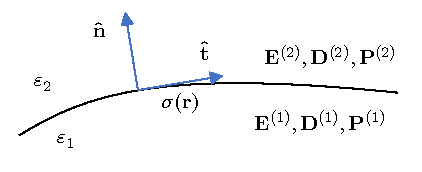
\includegraphics{bc_dielectrica.pdf}
	\caption{Übergang zwischen zwei Dielektrika. Die Felder $\vec E$, $\vec D$ und $\vec P$ ändern sich auf der Grenzfläche, an welcher sich eine Flächenladungsdichte $\sigma$ ausbildet. }
	\label{fig:bc_dielectrica}
\end{figure}

Für die Normalkomponente von $\vec {D}$ folgt aus $\divg \vec {D}=\rho _{\mathrm{Ma}}$
\begin{equation*}
	\hat{\vec {n}}\cdot \left(\vec {D}^{\left(2\right)}-\vec {D}^{\left(1\right)}\right)=D_{\perp }^{\left(2\right)}-D_{\perp }^{\left(1\right)}=\sigma
\end{equation*}
mit makroskopischer Flächenladungsdichte $\sigma $ auf der Grenzfläche\footnote{Für lineare, isotrope Dielektrika gilt insbesondere $\varepsilon _{2}E_{\perp }^{\left(2\right)}=\varepsilon _{1}E_{\perp }^{\left(1\right)}+\sigma .$}. Dieser Zusammenhang lässt sich mithilfe von $D_{\perp }^{\left(i\right)}=\varepsilon _{0}E_{\perp }^{\left(i\right)}+P_{\perp }^{\left(i\right)}$ auch kombiniert über das elektrische Feld und die Polarisation ausdrücken als
\begin{equation*}
	E_{\perp }^{\left(2\right)}-E_{\perp }^{\left(1\right)}=\frac{1}{\varepsilon _{0}}\left(\sigma +P_{\perp }^{\left(1\right)}-P_{\perp }^{\left(2\right)}\right).
\end{equation*}
Für den Spezialfall $\sigma =0$ wird in
\begin{align*}
	E_{\perp }^{\left(2\right)}-E_{\perp }^{\left(1\right)}=\frac{1}{\varepsilon _{0}}\left(P_{\perp }^{\left(1\right)}-P_{\perp }^{\left(2\right)}\right)\equiv \frac{1}{\varepsilon _{0}}\sigma _{p}
\end{align*}
die Polarisationsladung $\sigma _{p}$ definiert. Es gibt also aufgrund des Sprungs der Polarisation auf der Grenzfläche einen Sprung der Normalkomponente $E_{\perp }$. Das führt auf ein Brechungsgesetz (\Abbref{fig:dielectric_refraction}):

\begin{formal}
	Beim Übergang zum dielektrisch dünneren Medium wird das elektrische und das dielektrische Feld zum Lot hin gebrochen.
\end{formal}



\begin{figure}[htb]
	\centering
	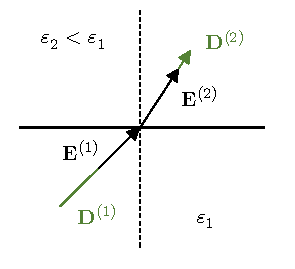
\includegraphics{dielectric_refraction.pdf}
	\caption{Die elektrischen Felder werden beim Übergang in Medien mit anderer Permittivität gebrochen, ähnlich zu der optischen Brechung. }
	\label{fig:dielectric_refraction}
\end{figure}

Diese Brechung ist ganz ähnlich zur optischen Brechung (wenn auch genau umgekehrt, denn dort wird das Licht beim Übergang in das optisch dichtere Medium zum Lot hin gebrochen). Es gilt
\begin{equation*}
	\vec {E}_{\parallel }^{\left(1\right)}=\vec {E}_{\parallel }^{\left(2\right)},\quad E_{\perp }^{\left(2\right)}=\frac{\varepsilon _{1}}{\varepsilon _{2}}E_{\perp }^{\left(1\right)}.
\end{equation*}
Diese Randbedingungen ermöglichen auch eine Messung von $\vec {D}$ und $\vec {E}$, indem eine Probeladung in einen schmalen Spalt im zu vermessenden Dielektrikum eingebracht wird, wie in \Abbref{fig:measure_fields_in_dielectricum} zu sehen.

\begin{figure}[htb]
	\centering
	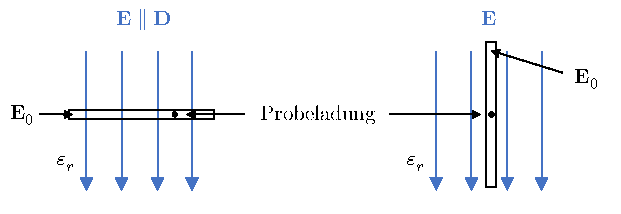
\includegraphics{measure_fields_in_dielectricum.pdf}
	\caption{Indem eine Probeladung in einem schmalen Spalt in ein Dielektrikum gebracht wird, können mithilfe der Randbedingungen die elektrischen Felder in diesem gemessen werden. Wird der Spalt senkrecht zu den Feldlinien gesetzt, so erfährt die Probeladung gerade die Kraft, die aus dem äußeren Feld $\vec E_0=\vec D/\varepsilon_0$ resultiert, was eine Messung der dielektrischen Verschiebung $\vec D$ ermöglicht. Bei einer parallelen Ausrichtung spürt die Ladung nur das Feld $\vec E_0=\vec E$. }
	\label{fig:measure_fields_in_dielectricum}
\end{figure}




\subsection{Entelektrisierungsfelder}


\begin{figure}[htb]
	\centering
	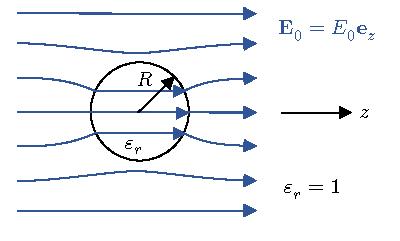
\includegraphics{dielectric_sphere_in_homogeneous_field.pdf}
	\caption{Eine dielektrische Kugel in einem ursprünglich homogenen äußeren Feld $\vec E_0$ beeinflusst die Feldlinien, weil die Randbedingungen erfüllt werden müssen. Innerhalb der Kugel ist das Feld homogen. }
	\label{fig:dielectric_sphere_in_homogeneous_field}
\end{figure}

Wird ein Dielektrikum einem äußeren elektrischen Feld $\vec {E}_{0}$ ausgesetzt, erzeugt die Polarisation ein sogenanntes Entelektrisierungs- oder Polarisationsfeld, welches das äußere Feld abschwächt. Der Grund sind Oberflächenladungen durch Polarisation.

Das Entelektrisierungsfeld soll exemplarisch für eine dielektrische Kugel in einem homogenen äußeren Feld berechnet werden (\Abbref{fig:dielectric_sphere_in_homogeneous_field}).

Da es keine freien Ladungen gibt, also $\rho _{\mathrm{Ma}}=0$, ist die Laplace-Gleichung $\nabla ^{2}\phi =0$ zu lösen. Aufgrund der Axialsymmetrie um die $z$-Achse wird als Lösungsansatz eine Linearkombination aus Legendre-Polynomen erster Ordnung für die Beschreibung der Potentiale $\phi _{i}$ innerhalb und $\phi _{a}$ außerhalb der Kugel verwendet:
\begin{equation*}
	\phi _{i,a}=\sum _{l=0}^{\infty }\left(a_{l}^{\left(i,a\right)}r^{l}+b_{l}^{\left(i,a\right)}r^{-\left(l+1\right)}\right)P_{l}\left(\cos \vartheta \right)
\end{equation*}
Aus Betrachtungen für die Grenzfälle können die Koeffizienten $a_{l}^{\left(i,a\right)}$ und $b_{l}^{\left(i,a\right)}$ ermittelt werden:

\begin{enumerate}[i)]
	\item Im Unendlichen ($r\rightarrow \infty $) verschwindet die Störung durch die dielektrische Kugel und das Feld ist homogen, $E_{0}\vec {e}_{z}=-\nabla \phi _{a}$. Das Potential nimmt dort also die Form $\phi _{a}\left(r\rightarrow \infty \right)=-E_{0}z=-E_{0}r\cos \vartheta $ an. Durch einen Koeffizientenvergleich erhält man $a_{1}^{\left(a\right)}=-E_{0}, a_{l>1}^{\left(a\right)}=0$.

	\item Im Mittelpunkt ($r=0$) darf das Potential nicht divergieren, sodass $b_{l}^{\left(i\right)}=0$ für alle $l$.

	\item An der Grenzfläche ($r=R$) muss gelten, dass $E_{\parallel }^{\left(i\right)}=E_{\parallel }^{\left(a\right)}$ und $\varepsilon _{r}E_{\perp }^{\left(i\right)}=E_{\perp }^{\left(a\right)}$. Einsetzen und Lösen des Gleichungssystems führt auf
	      \begin{equation*}
		      a_{1}^{\left(i\right)}=-\frac{3}{\varepsilon _{r}+2}E_{0},\quad b_{1}^{\left(a\right)}=\frac{\varepsilon _{r}-1}{\varepsilon _{r}+2}R^{3}E_{0},\quad a_{l>1}^{\left(i\right)}=0,\quad b_{l>1}^{\left(a\right)}=0.
	      \end{equation*}
\end{enumerate}

Mit den Ersetzungen $r\cos \vartheta =z=\vec {r}\cdot \vec {e}_{z}$ und dem Dipolmoment $\vec {p}=\frac{4}{3}\pi R^{3}\vec {P}$ erhält man schließlich
\begin{equation*}
	\phi _{i}=-\frac{3}{\varepsilon _{r}+2}\vec {E}_{0}\cdot \vec {r}, \quad\phi _{a}=-\vec {E}_{0}\cdot \vec {r}+\frac{1}{4\pi \varepsilon _{0}}\frac{\vec {p}\cdot \vec {r}}{r^{3}}
\end{equation*}
und
\begin{equation*}
	\vec {E}^{\left(i\right)}=\frac{3}{\varepsilon _{r}+2}\vec {E}_{0}, \quad\vec {E}^{\left(a\right)}=\vec {E}_{0}-\frac{1}{4\pi \varepsilon _{0}}\nabla \frac{\vec {p}\cdot \vec {r}}{r^{3}}.
\end{equation*}
Im Innern der Kugel ist also das elektrische Feld homogen und die (lineare) Polarisation ist
\begin{equation*}
	\vec {P}=\varepsilon _{0}\chi \vec {E}^{\left(i\right)}=3\varepsilon _{0}\frac{\varepsilon _{r}-1}{\varepsilon _{r}+2}\vec {E}_{0}.
\end{equation*}
Das innere Feld lässt sich auch umformulieren zu
\begin{equation*}
	\vec {E}^{\left(i\right)}=\vec {E}_{0}-\frac{1}{3\varepsilon _{0}}\vec {P},
\end{equation*}
also der Summe des ursprünglichen äußeren Feldes und eines abschwächenden Feldes $\vec {E}'\equiv \vec {P}/3\varepsilon _{0}$ \textendash{} dem abschirmenden Entelektrisierungsfeld (\Abbref{fig:dielectric_ball_polarisation_field}).

\begin{figure}[htb]
	\centering
	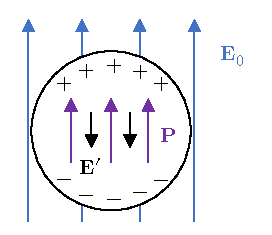
\includegraphics{dielectric_ball_polarisation_field.pdf}
	\caption{Entelektrisierungsfeld/Polarisationsfeld einer dielektrischen Kugel in einem homogenen äußeren elektrischen Feld. }
	\label{fig:dielectric_ball_polarisation_field}
\end{figure}


Für den allgemeinen, nicht kugelsymmetrischen Fall sind Entelektrisierungsfeld $\vec {E}'$ und Polarisation nicht parallel. Dann gilt
\begin{equation*}
	\vec {E}'=-\frac{1}{\varepsilon _{0}}\lambda \vec {P}
\end{equation*}


\begin{figure}[htb]
	\centering
	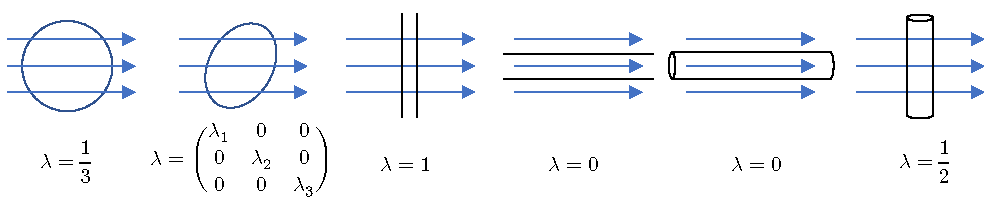
\includegraphics{simple_dielectric_bodies_polarisation_field.pdf}
	\caption{}
	\label{fig:simple_dielectric_bodies_polarisation_field}
\end{figure}

mit dem Entelektrisierungstensor $\lambda$. Für die Kugel ist natürlich $\lambda =1/3$, für eine zum äußeren Feld orthogonale Platte dagegen $\lambda =1$ und für eine zum äußeren Feld parallele Platte $\lambda =0$. Für einen langen Zylinder, der orthogonal zum Feld steht ist $\lambda =1/2$ (siehe \Abbref{fig:simple_dielectric_bodies_polarisation_field}).

Für komplexere dielektrische Körper in einem homogenen äußeren Magnetfeld ist $\vec {P}$ nicht homogen.



\subsection{Clausius-Mosotti-Formel}

Im Kapitel \ref{sec:Makroskopische_Gleichungen_der_Elektrostatik} wurde bereits die molekulare Polarisierbarkeit $\alpha $ eingeführt. Diese beschreibt das induzierte Dipolmoment eines Moleküls in Abhängigkeit von dem lokalen elektrischen Feld
\begin{equation*}
	\vec {p}=\varepsilon _{0}\alpha \vec {E}_{\mathrm{loc}}.
\end{equation*}
Die Clausius-Mosotti-Formel beschreibt, wie die molekulare Polarisierbarkeit mit der (makroskopischen) Dielektrizität $\varepsilon _{r}$ zusammenhängt:
\begin{equation*}
	\frac{\varepsilon _{r}-1}{\varepsilon _{r}+2}=\frac{1}{3}n\alpha
\end{equation*}

\begin{figure}[htb]
	\centering
	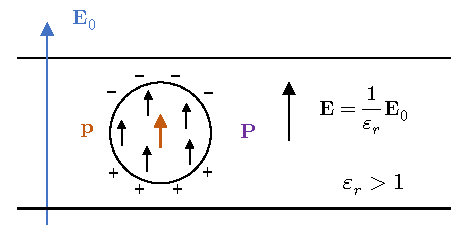
\includegraphics{clausius_mosotti.pdf}
	\caption{Ein Dipol $\vec p$ befindet sich in einem Medium mit $\varepsilon_r >1$. Ein äußeres elektrisches Feld $\vec E_0$ liegt an (lokal homogen). Im Dielektrikum ist die Feldstärke $\vec E=\vec E_0/\varepsilon_r$. Es wird ein kleiner, kugelförmiger Bereich um den Dipol herum betrachtet, innerhalb dessen alle Dipole des Mediums berücksichtigt werden. Der Dipol $\vec p$ ruft eine Polarisation $\vec P$ hervor. }
	\label{fig:clausius_mosotti}
\end{figure}

Die Formel wird hergeleitet aus der in \Abbref{fig:clausius_mosotti} dargestellten Geometrie. Ein äußeres elektrisches Feld $\vec {E}_{0}$ durchdringt das Medium mit $\varepsilon _{r}>1$. Dort ist also das Feld $\vec {E}=\vec {E}_{0}/\varepsilon _{r}$. Im Medium befindet sich ein mikroskopischer Dipol $\vec {p}$. Durch dessen Existenz ist auch eine Polarisation $\vec {P}$ vorhanden, die das Feld innerhalb des Mediums verändert. Um jetzt das lokale Feld beim Dipol zu bestimmen, legen wir eine kleine Hohlkugel um den Dipol herum. Außerhalb dieser Kugel rechnen wir makroskopisch mit der Polarisation, aber innerhalb der Kugel betrachten wir vorsichtshalber die einzelnen Dipole des Dielektrikums (z.B. Dipole auf Gitterplätzen im Festkörper). Der Bereich außerhalb ist also das kontinuierliche Dielektrikum, während innen diskrete Dipole liegen.

Das lokale elektrische Feld hat verschiedene Beiträge: zum einen das Feld $\vec {E}$ im Medium, dann das Feld, das durch die Oberflächenladung (von der Polarisation erzeugt) an der Kugel hervorgerufen wird (sog. Lorentzfeld) und schließlich das Feld, das aus den Dipolen um $\vec {p}$ herum resultiert:
\begin{equation*}
	\vec {E}_{\mathrm{loc}}=\vec {E}+\vec {E}_{\sigma }+\vec {E}_{\mathrm{dip}}
\end{equation*}
Die zweite Komponente lässt sich sofort bestimmen, da es genau dem Entelektrisierungsfeld $\frac{1}{3\varepsilon _{0}}\vec {P}$ entspricht, nur mit verkehrtem Vorzeichen, weil das Dielektrikum jetzt außerhalb der Kugel liegt und nicht innerhalb. Für kubische Gitter, Flüssigkeiten und Gase ist aufgrund der Isotropie $\vec {E}_{\mathrm{dip}}=0$.

Damit kann die Polarisation über die Dipoldichte $n$ ausgerechnet werden:
\begin{equation*}
	\vec {P} =n\vec {p}=\varepsilon _{0}n\alpha \vec {E}_{\mathrm{loc}}=\varepsilon _{0}n\alpha \left(\vec {E}+\frac{1}{3\varepsilon _{0}}\vec {P}\right)
\end{equation*}
Diese Gleichung kann umgestellt und mit $\vec {P}=\varepsilon _{0}\chi \vec {E}$ verglichen werden, sodass man
\begin{equation*}
	\chi =\frac{n\alpha }{1-\frac{1}{3}n\alpha }
\end{equation*}
bzw.
\begin{equation*}
	\varepsilon _{r}=1+\chi =\frac{1+\frac{2}{3}n\alpha }{1-\frac{1}{3}n\alpha }
\end{equation*}
erhält. Umformen führt dann auf die Clausius-Mosotti-Formel,
\begin{equation*}
	\frac{\varepsilon _{r}-1}{\varepsilon _{r}+2}=\frac{1}{3}n\alpha ,
\end{equation*}
die eine nichtlineare Beziehung zwischen $\varepsilon _{r}$ und $\alpha $ beschreibt\footnote{In der Optik ist diese Formel ebenfalls von Bedeutung. Sie wird dort für den Brechungsindex $\overline{n}=\sqrt{\varepsilon _{r}}$ geschrieben und als Lorenz-Lorentz-Formel bezeichnet. }.

Für Gase ($n\alpha \ll 1$) ist
\begin{equation*}
	\chi =n\alpha \implication \varepsilon _{r}=1+n\alpha ,
\end{equation*}
die Beziehung wird also linear aufgrund der Vernachlässigung des Lorentzfeldes $\vec {E}_{\sigma }$. In allgemeinen (nicht kubischen) Kristallen spielen die Beiträge von $\vec {E}_{\mathrm{dip}}$ allerdings eine Rolle.

\section{Elektrostatische Energie im Dielektrikum}

Die (Selbst-) Energie einer makroskopischen Ladungsverteilung $\rho =\rho _{\mathrm{Ma}}$ im Vakuum ist bekanntermaßen
\begin{equation*}
	U_{\text{Selbst}}=\frac{1}{2}\int \diffa[3]{\vec{r}}\rho \left(\vec {r}\right)\phi \left(\vec {r}\right)
\end{equation*}
und entspricht gerade der Arbeit, die aufzubringen ist, um die Ladungsverteilung aus dem Unendlichen zusammenzubringen. Im Dielektrikum verändert sich diese Energie, weil es auch Arbeit kostet, die Polarisation im Dielektrikum zu erzeugen.

Die Berechnung erfolgt analog zu der im Vakuum. Die Änderung von $U$ durch Hinzufügen einer zusätzlichen Ladungsdichte $\delta \rho $ bei $\phi \left(\vec {r}\right)$ berechnet sich durch
\begin{equation*}
	\delta U=\int _{V}\diffa[3]{\vec{r}}\phi \left(\vec {r}\right)\delta \rho \left(\vec {r}\right).
\end{equation*}
Mit $\nabla \cdot \vec {D}=\rho \implication \delta \rho =\nabla \cdot \delta \vec {D}$ und partieller Integration folgt
\begin{equation*}
	\delta U=\int _{V}\diffa[3]{\vec{r}}\phi \left(\vec {r}\right)\nabla \cdot \delta \vec {D}=\int _{\partial V}\phi \left(\vec {r}\right)\delta \vec {D}\cdot \diff \vec {S}-\int _{V}\diffa[3]{\vec{r}}\nabla \phi \left(\vec {r}\right)\delta \vec {D}=\int \diffa[3]{\vec{r}}\vec {E}\left(\vec {r}\right)\cdot \delta \vec {D}.
\end{equation*}
Das Volumen kann so gewählt werden, dass das Dielektrikum gänzlich innerhalb liegt, sodass der Oberflächenterm bei der partiellen Integration verschwindet.

Im linearen Dielektrikum, $\vec {D}=\varepsilon _{0}\varepsilon _{r}\vec {E}\implication \vec {E}\cdot \delta \vec {D}=\frac{1}{2}\delta \left(\vec {E}\cdot \vec {D}\right)$, erhält man durch Integration (Einbringen der ganzen Ladungsdichte $\rho _{\mathrm{Ma}}$ in das Medium)\footnote{Diese Gleichung hat dieselbe Form wie die im Vakuum, nur dass jetzt die makroskopische Ladungsdichte $\rho _{\mathrm{Ma}}$ als Summe der gemittelten freien Ladungsdichte und Monopoldichte eingesetzt wird. }
\begin{equation*}
	U_{\text{Selbst}}=\frac{1}{2}\int \diffa[3]{\vec{r}}\vec {E}\cdot \vec {D}=\frac{1}{2}\int \diffa[3]{\vec{r}}\rho _{\mathrm{Ma}}\left(\vec {r}\right)\phi \left(\vec {r}\right)
\end{equation*}
bzw. (wieder mit partieller Integration)
\begin{equation*}
	U_{\text{Selbst}}=-\frac{1}{2}\int \diffa[3]{\vec{r}}\nabla \phi \left(\vec {r}\right)\cdot D=\frac{1}{2}\int \diffa[3]{\vec{r}}\phi \left(\vec {r}\right)\nabla \cdot \vec {D}.
\end{equation*}
Die schon hergeleitete Formel
\begin{equation*}
	u=\frac{1}{2}\vec {E}\cdot \vec {D}
\end{equation*}
für die Energiedichte gilt für lineare Dielektrika genauso wie für das Vakuum.

Nun soll noch der Fall betrachtet werden, in dem ein lineares Dielektrikum in ein bereits bestehendes Feld $\vec {E}_{0}$ eingebracht wird. Hier gilt jetzt
\begin{equation*}
	U=-\frac{1}{2}\int \diffa[3]{\vec{r}}\vec {P}\cdot \vec {E}_{0}.
\end{equation*}
Das entspricht also gerade der Dipolenergie von $\vec P\diffa[3]{\vec{r}}$ im Feld $\vec {E}_{0}$. Der Faktor $1/2$ kommt zustande, weil die Polarisation $\vec {P}$ durch das äußere Feld erst induziert wird.

Außerdem wird das Dielektrikum in Gebiete mit stärkerem Feld oder höherer Polarisation gezogen, weil dann die potentielle Energie abnimmt. Die wirkende Kraft berechnet sich aus dem Potential,
\begin{equation*}
	\vec {F}=\nabla U.
\end{equation*}
Dieses Prinzip findet eine sehr wichtige Anwendung in der optischen Pinzette.

